\section{Modified AODV Routing Protocol}
\subsection{Proposed Algorithm}
The below Algorithm is proposed by The paper:


A new field will be added in
the RREQ for calculating transmission energy. The format of
the new RREQ will be


<source\_address, dest\_sequence\_id, source\_sequence\_id,
broadcast\_id, dest\_address, hop\_count, transmission\_energy>
Now based on each packets Transmission energy:
\begin{algorithmic}
\State Calculate drop factor d for every transmitting node.
\State Generate a random number between $0 and 1.$
\If {$random\_value > drop factor$}
    \State broadcast/forward RREQ\_packet,
\Else
\State drop RREQ\_packet.
\EndIf
\end{algorithmic}
This algorithm has some major problem. It always drop packet when network isn't congested at all.
I propose a modification on this algorithm. The idea is to count last $d$ seconds RREQ packet number and drop packet if number of packet cross the average.

\begin{algorithmic}
\State $average \gets get\_average\_per\_second()$
\State $number\_of\_packet\_in\_last\_second \gets get\_last\_second\_count()$
\State Calculate drop factor d for every transmitting node.
\State Generate a random number between 0 and 1.
\If {$number\_of\_packet\_in\_last\_second < average \And random\_value > drop factor$}
    \State broadcast/forward RREQ\_packet,
\Else
\State drop RREQ\_packet.
\EndIf
\end{algorithmic}

\subsection{Implementation}
The following code is added to aodv.cc in AODV::recvRequest(Packet *p) function:
\begin{lstlisting}[language=c]
int flag = 0;
 while(current_time< (int)CURRENT_TIME){
    current_time++;
    for(int i=0;i<MAX_SECOND-1;i++){
      rreq_count[i]  = rreq_count[i+1] ;
    }
    rreq_count[MAX_SECOND-1] = 0;
 }
  rreq_count[MAX_SECOND-1]++;
 // calculating average rreq count
  int sum = 0;
  for(int i=0;i<MAX_SECOND;i++){
    sum += rreq_count[i];
  }
  double avg = (double)sum/MAX_SECOND;
  // drop if high rreq count
  if(avg<rreq_count[MAX_SECOND-1]){
    flag = 1;
  }
// drop if low energy
double drop_prob = 1.0 - 
    (double)rq->rq_transmission_energy/AODV_MAX_TRANSMISSION_ENERGY;
// decrease Transmission Energy
if(rq->rq_transmission_energy>1){
  rq->rq_transmission_energy--;
}

/* -------- more code ----*/
/*
  * Can't reply. So forward the  Route Request
  */
 else {
 	if((Random::uniform() < drop_prob) && flag==1){
  	Packet::free(p);
  	fprintf(stderr,"freeing packet\n");
  	return;
	}
   ih->saddr() = index;
   ih->daddr() = IP_BROADCAST;
   rq->rq_hop_count += 1;
   // Maximum sequence number seen en route
   if (rt) rq->rq_dst_seqno = max(rt->rt_seqno, rq->rq_dst_seqno);
   forward((aodv_rt_entry*) 0, p, DELAY);
 }
\end{lstlisting}
While sending a packet initially, I set the energy to a certain value.
Code in AODV::sendRequest(nsaddr\_t dst)
\begin{lstlisting}
 // Fill up some more fields. 
 rq->rq_type = AODVTYPE_RREQ;
 rq->rq_hop_count = 1;
 rq->rq_bcast_id = bid++;
 rq->rq_dst = dst;
 rq->rq_dst_seqno = (rt ? rt->rt_seqno : 0);
 rq->rq_src = index;
 seqno += 2;
 rq->rq_transmission_energy= AODV_MAX_TRANSMISSION_ENERGY;
 assert ((seqno%2) == 0);
 rq->rq_src_seqno = seqno;
 rq->rq_timestamp = CURRENT_TIME;
\end{lstlisting}
And the new packet Type -> Code snipped from packet.h
\begin{lstlisting}
struct hdr_aodv_request {
    u_int8_t        rq_type;	// Packet Type
    u_int8_t        reserved[2];
    u_int8_t        rq_hop_count;   // Hop Count
    u_int32_t       rq_bcast_id;    // Broadcast ID

    nsaddr_t        rq_dst;         // Destination IP Address
    u_int32_t       rq_dst_seqno;   // Destination Sequence Number
    nsaddr_t        rq_src;         // Source IP Address
    u_int32_t       rq_src_seqno;   // Source Sequence Number
        
    u_int8_t        rq_transmission_energy; // Transmission Energy

    double          rq_timestamp;   // when REQUEST sent;
}
\end{lstlisting}
\subsection{Results}
\subsubsection{Description of the simulation}
The simulation is based on the IEEE 802.11.2(mobile) standard. Routing is based on the aodv protocol. The simulation is based on the ns-2 simulator. The simulation is based on the following parameters:
\begin{itemize}
    \item Channel: Wireless channel
    \item Propagation: Two-ray ground
    \item Antenna: Omnidirectional
    \item Link: IEEE 802.11.2
    \item Queue: Drop-tail
    \item Routing: AODV
    \item Mobility: Random waypoint
    \item Position: Grid
    \item Area: 1000 x 1000 meters
    \item Flow: Random source to random destination
    \item Packet size: 64 bytes
    \item Number of nodes: Variable
    \item Number of flows: Variable
    \item Packet rate: Variable
    \item Speed: Variable
    \item Simulation time: 60 seconds
\end{itemize}
\subsubsection{Results}
Varying Number of Node.
Baseline parameters are as follows:
\begin{itemize}
    \item Number of flows: 20
    \item Packet rate: 100 packets per second
    \item Speed: 5 meters per second
\end{itemize}
The number of nodes is varied from 20 to 100 in steps of 20.
See Figure \ref{node_throughput_modified} ,\ref{node_delay_modified} , \ref{node_delivery_modified} , \ref{node_drop_modified}, \ref{node_energy_modified} and \ref{node_energy_modified_per_byte}  for the result.
\begin{figure}[h]
\begin{subfigure}{.5\textwidth}
  \centering
  % include first image
  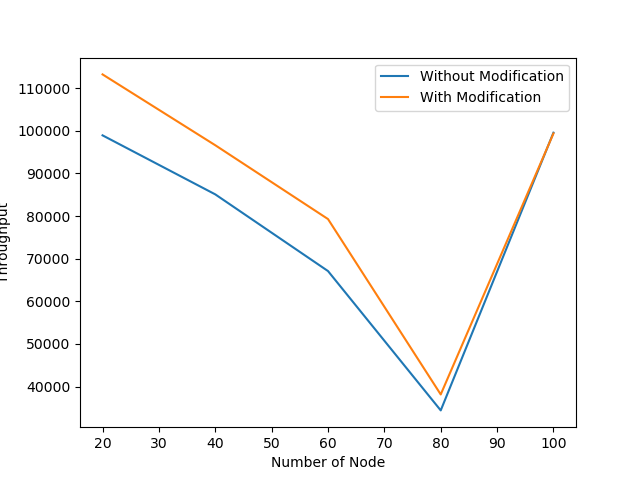
\includegraphics[width=.8\linewidth]{modified_fig/NumberofNodevsThroughput.png}
     \caption{Number of Nodes Vs Throughput}
    \label{node_throughput_modified}
\end{subfigure}
\begin{subfigure}{.5\textwidth}
  \centering
  % include second image
  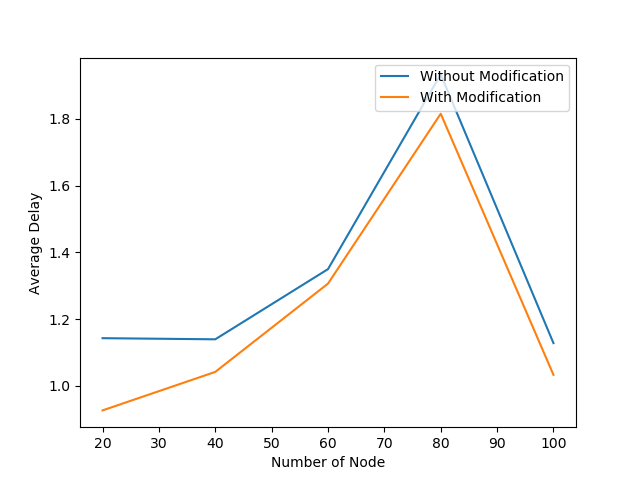
\includegraphics[width=.8\linewidth]{modified_fig/NumberofNodevsAverageDelay.png}
    \caption{Number of Nodes Vs Average Delay}
     \label{node_delay_modified}
\end{subfigure}
\begin{subfigure}{.5\textwidth}
  \centering
  % include third image
  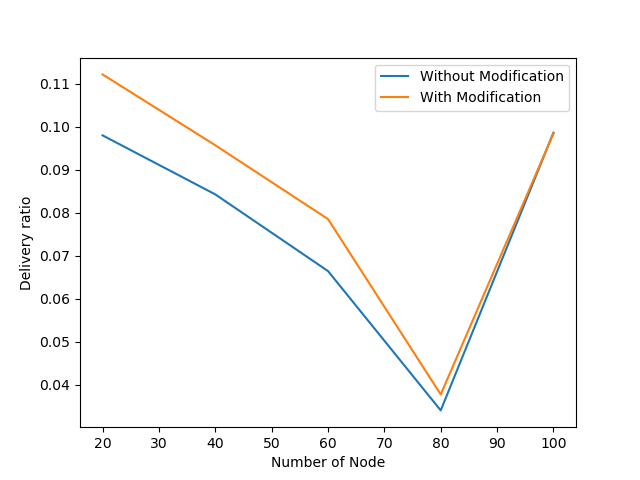
\includegraphics[width=.8\linewidth]{modified_fig/NumberofNodevsDeliveryRatio.png}
     \caption{Number of Nodes Vs Delivary Ratio}
     \label{node_delivery_modified}
\end{subfigure}
\begin{subfigure}{.5\textwidth}
  \centering
  % include fourth image
  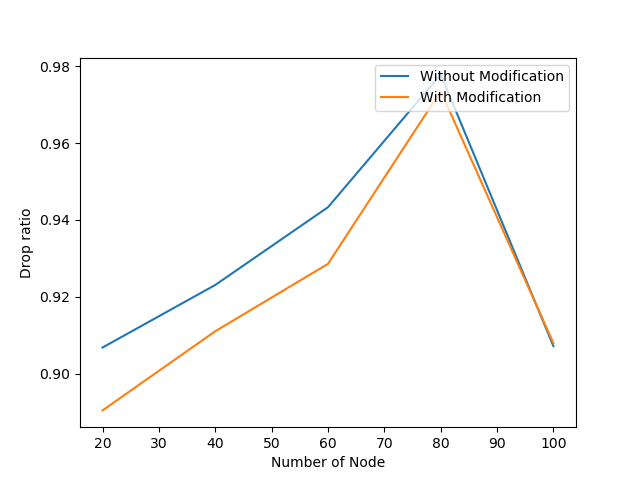
\includegraphics[width=.8\linewidth]{modified_fig/NumberofNodevsDropRatio.png}
     \caption{Number of Nodes Vs Drop Ratio}
     \label{node_drop_modified}
\end{subfigure}
\begin{subfigure}{.5\textwidth}
  \centering
  % include fifth image
  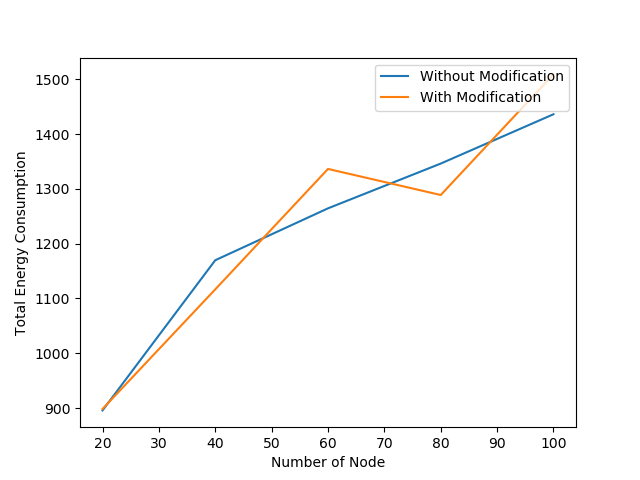
\includegraphics[width=.8\linewidth]{modified_fig/NumberofNodevsTotalEnergyConsumption.png}
     \caption{Number of Nodes Vs Energy Consumption}
     \label{node_energy_modified}
\end{subfigure}
\begin{subfigure}{.5\textwidth}
  \centering
  % include sixth image
  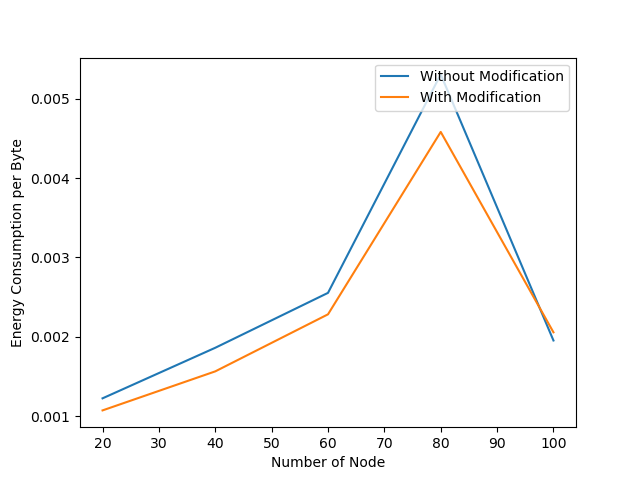
\includegraphics[width=.8\linewidth]{modified_fig/NumberofNodevsEnergyConsumptionperByte.png}
     \caption{Number of Nodes Vs Energy Per Byte}
     \label{node_energy_modified_per_byte}
\end{subfigure}
\caption{Varying Number of Nodes}
\label{fig:varyingNode}
\end{figure}

Varying Number of Flows.
Baseline parameters are as follows:
\begin{itemize}
    \item Number of nodes: 60
    \item Packet rate: 100 packets per second
    \item Speed: 5 meters per second
\end{itemize}
The number of flows is varied from 10 to 50 in steps of 10.
See Figure \ref{flow_throughput_modified} ,\ref{flow_delay_modified} , \ref{flow_delivery_modified} , \ref{flow_drop_modified}, \ref{flow_energy_modified} and \ref{flow_energy_modified_per_byte} for the result.
\begin{figure}[h]
\begin{subfigure}{.5\textwidth}
  \centering
  % include first image
  \includegraphics[width=.8\linewidth]{modified_fig/NumberofFlowvsThroughput.png}
     \caption{Number of Flows Vs Throughput}
    \label{flow_throughput_modified}
\end{subfigure}
\begin{subfigure}{.5\textwidth}
  \centering
  % include second image
  \includegraphics[width=.8\linewidth]{modified_fig/NumberofFlowvsAverageDelay.png}
    \caption{Number of Flows Vs Average Delay}
     \label{flow_delay_modified}
\end{subfigure}
\begin{subfigure}{.5\textwidth}
  \centering
  % include third image
  \includegraphics[width=.8\linewidth]{modified_fig/NumberofFlowvsDeliveryRatio.png}
     \caption{Number of Flows Vs Delivary Ratio}
     \label{flow_delivery_modified}
\end{subfigure}
\begin{subfigure}{.5\textwidth}
  \centering
  % include fourth image
  \includegraphics[width=.8\linewidth]{modified_fig/NumberofFlowvsDropRatio.png}
     \caption{Number of Flows Vs Drop Ratio}
     \label{flow_drop_modified}
\end{subfigure}
\begin{subfigure}{.5\textwidth}
  \centering
  % include fifth image
  \includegraphics[width=.8\linewidth]{modified_fig/NumberofFlowvsTotalEnergyConsumption.png}
     \caption{Number of Flows Vs Energy Consumption}
     \label{flow_energy_modified}
\end{subfigure}
\begin{subfigure}{.5\textwidth}
  \centering
  % include sixth image
  \includegraphics[width=.8\linewidth]{modified_fig/NumberofFlowvsEnergyConsumptionperByte.png}
     \caption{Number of Flows Vs Energy Per Byte}
     \label{flow_energy_modified_per_byte}
\end{subfigure}
\caption{Varying Number of Flows}
\label{fig:varyingFlow}
\end{figure}


Varying Packet per Second.Baseline parameters are as follows:
\begin{itemize}
    \item Number of nodes: 60
    \item Number of flows: 10
    \item Speed: 5 meters per second
\end{itemize}
The packet rate is varied from 100 to 500 packets per second in steps of 100.
See Figure \ref{packet_rate_throughput_modified} ,\ref{packet_rate_delay_modified} , \ref{packet_rate_delivery_modified} , \ref{packet_rate_drop_modified}, \ref{packet_rate_energy_modified} and \ref{packet_rate_energy_modified_per_byte}  for the result.
\begin{figure}[h]
\begin{subfigure}{.5\textwidth}
  \centering
  % include first image
  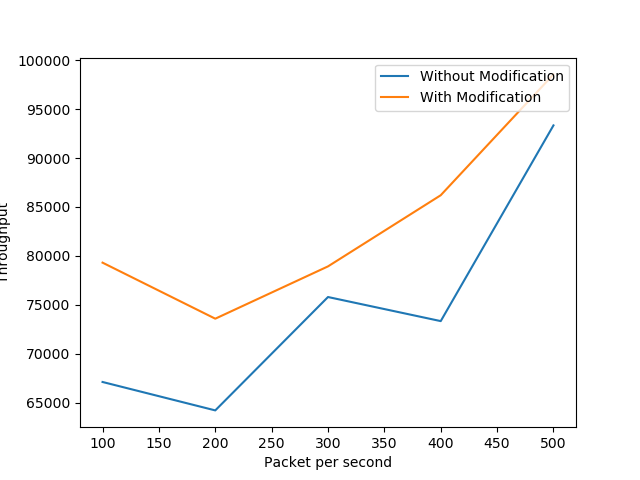
\includegraphics[width=.8\linewidth]{modified_fig/PacketpersecondvsThroughput.png}
     \caption{Packet Rate Vs Throughput}
    \label{packet_rate_throughput_modified}
\end{subfigure}
\begin{subfigure}{.5\textwidth}
  \centering
  % include second image
  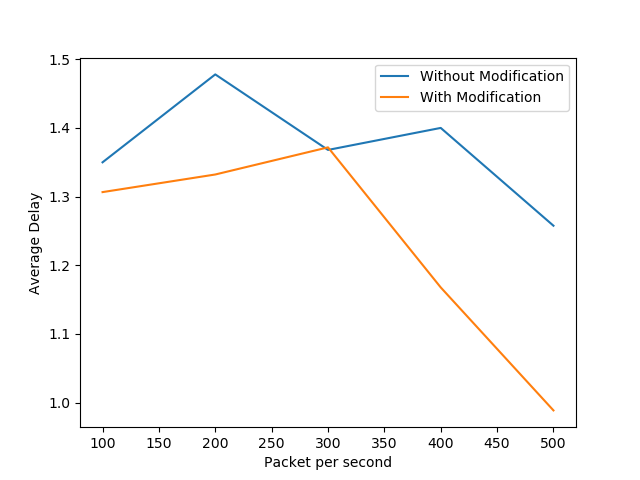
\includegraphics[width=.8\linewidth]{modified_fig/PacketpersecondvsAverageDelay.png}
    \caption{Packet Rate Vs Average Delay}
     \label{packet_rate_delay_modified}
\end{subfigure}
\begin{subfigure}{.5\textwidth}
  \centering
  % include third image
  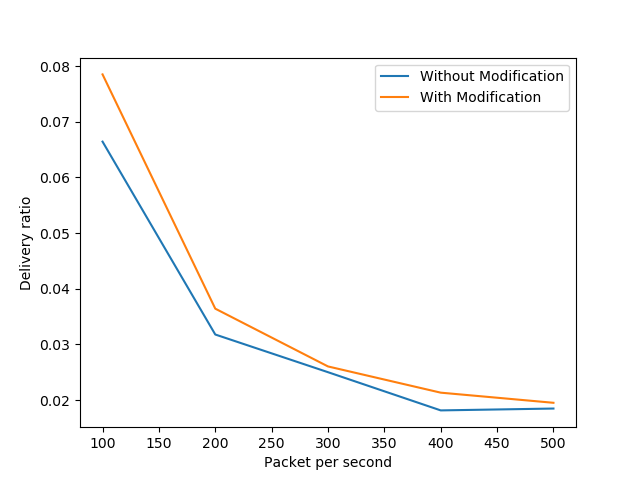
\includegraphics[width=.8\linewidth]{modified_fig/PacketpersecondvsDeliveryRatio.png}
     \caption{Packet Rate Vs Delivary Ratio}
     \label{packet_rate_delivery_modified}
\end{subfigure}
\begin{subfigure}{.5\textwidth}
  \centering
  % include fourth image
  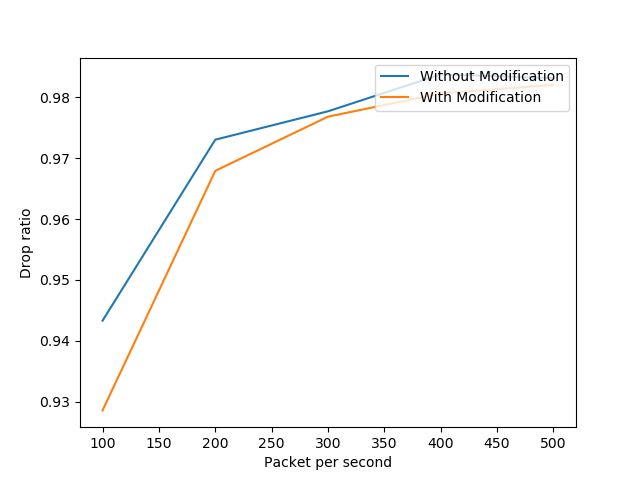
\includegraphics[width=.8\linewidth]{modified_fig/PacketpersecondvsDropRatio.png}
     \caption{Packet Rate Vs Drop Ratio}
     \label{packet_rate_drop_modified}
\end{subfigure}
\begin{subfigure}{.5\textwidth}
  \centering
  % include fifth image
  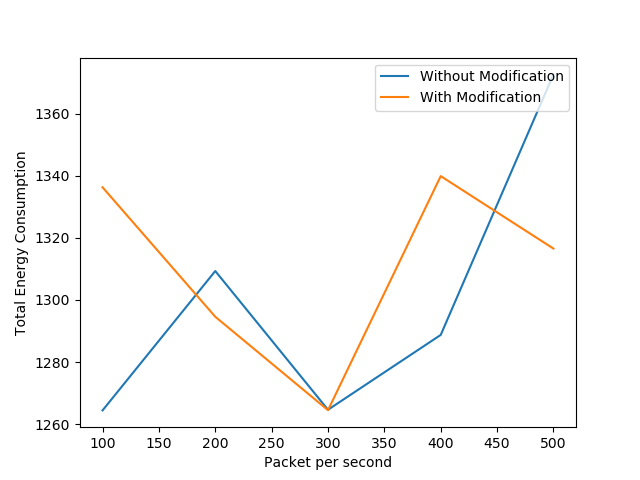
\includegraphics[width=.8\linewidth]{modified_fig/PacketpersecondvsTotalEnergyConsumption.png}
     \caption{Packet Rate Vs Energy Consumption}
     \label{packet_rate_energy_modified}
\end{subfigure}
\begin{subfigure}{.5\textwidth}
  \centering
  % include sixth image
  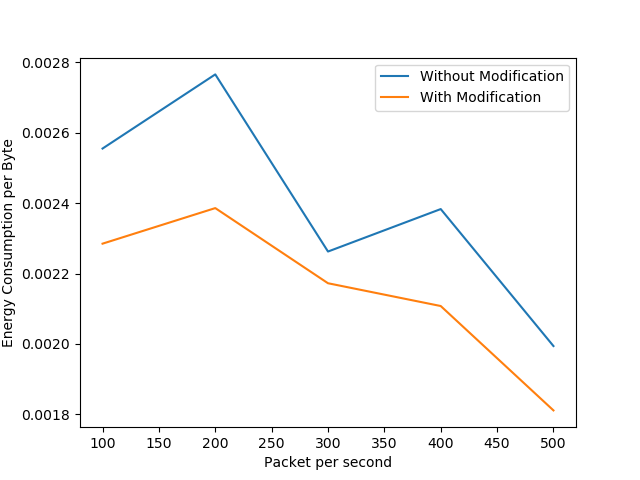
\includegraphics[width=.8\linewidth]{modified_fig/PacketpersecondvsEnergyConsumptionperByte.png}
     \caption{Packet Rate Vs Energy Per Byte}
     \label{packet_rate_energy_modified_per_byte}
\end{subfigure}
\caption{Varying Packet Rate}
\label{fig:varyingPacketRate}
\end{figure}

Varying Speed.
Baseline parameters are as follows:
\begin{itemize}
    \item Number of nodes: 60
    \item Number of flows: 20
    \item Packet Rate: 100 packets per second
\end{itemize}
The speed is varied from 5 to 25 meters per second in steps of 5.
See Figure \ref{speed_throughput_modified} ,\ref{speed_delay_modified} , \ref{speed_delivery_modified} , \ref{speed_drop_modified}, \ref{speed_energy_modified} and \ref{speed_energy_modified_per_byte}  for the result.
\begin{figure}[h]
\begin{subfigure}{.5\textwidth}
  \centering
  % include first image
  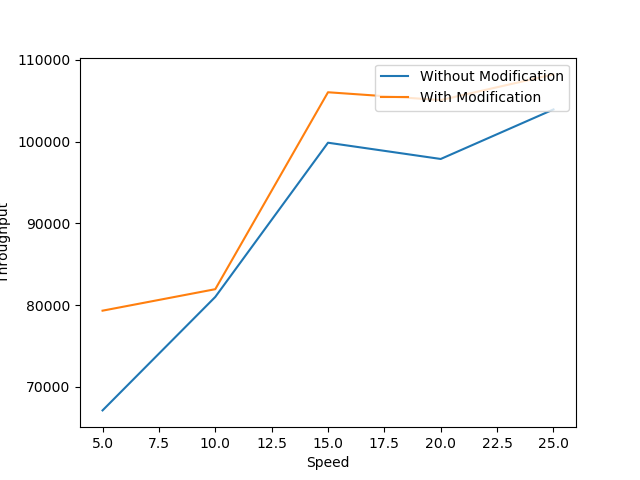
\includegraphics[width=.8\linewidth]{modified_fig/SpeedvsThroughput.png}
     \caption{Speed Vs Throughput}
    \label{speed_throughput_modified}
\end{subfigure}
\begin{subfigure}{.5\textwidth}
  \centering
  % include second image
  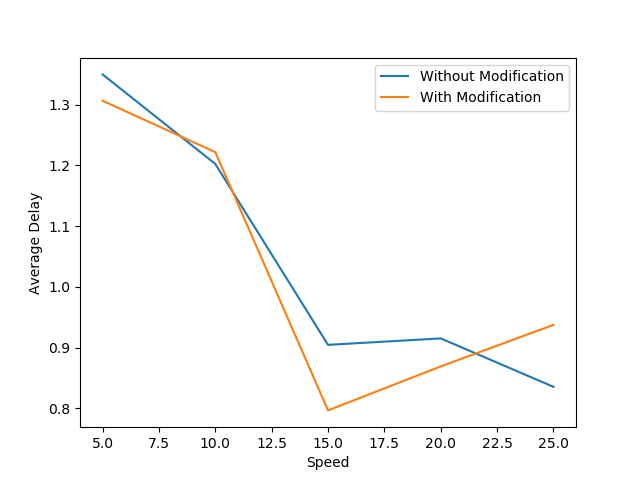
\includegraphics[width=.8\linewidth]{modified_fig/SpeedvsAverageDelay.png}
    \caption{Speed Vs Average Delay}
     \label{speed_delay_modified}
\end{subfigure}
\begin{subfigure}{.5\textwidth}
  \centering
  % include third image
  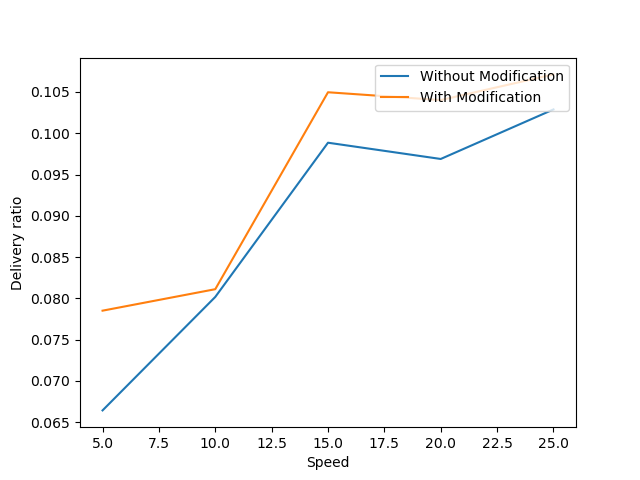
\includegraphics[width=.8\linewidth]{modified_fig/SpeedvsDeliveryRatio.png}
     \caption{Speed Vs Delivary Ratio}
     \label{speed_delivery_modified}
\end{subfigure}
\begin{subfigure}{.5\textwidth}
  \centering
  % include fourth image
  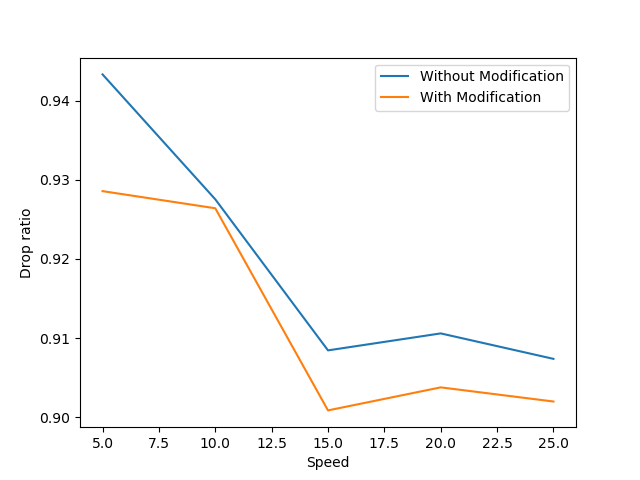
\includegraphics[width=.8\linewidth]{modified_fig/SpeedvsDropRatio.png}
     \caption{Speed Vs Drop Ratio}
     \label{speed_drop_modified}
\end{subfigure}
\begin{subfigure}{.5\textwidth}
  \centering
  % include fifth image
  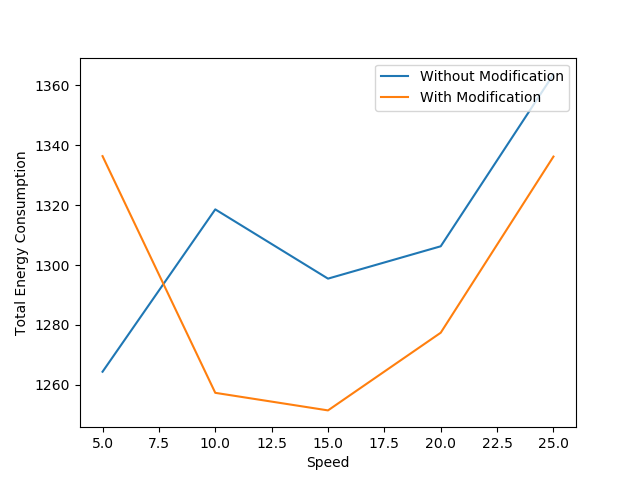
\includegraphics[width=.8\linewidth]{modified_fig/SpeedvsTotalEnergyConsumption.png}
     \caption{Speed Vs Energy Consumption}
     \label{speed_energy_modified}
\end{subfigure}
\begin{subfigure}{.5\textwidth}
  \centering
  % include sixth image
  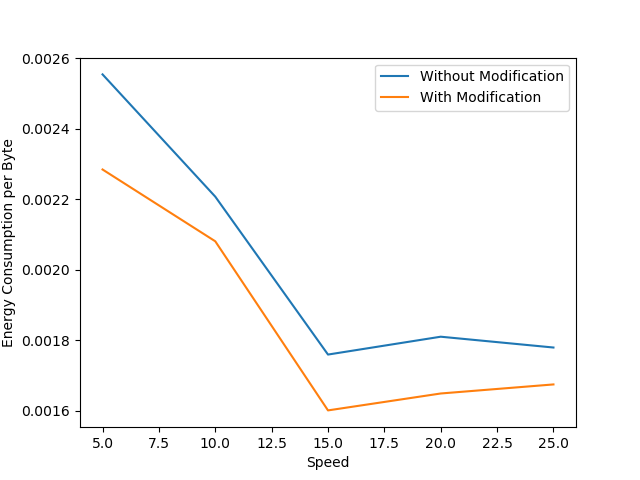
\includegraphics[width=.8\linewidth]{modified_fig/SpeedvsEnergyConsumptionperByte.png}
     \caption{Speed Vs Energy Per Byte}
     \label{speed_energy_modified_per_byte}
\end{subfigure}
\caption{Varying Speed}
\label{fig:varyingSpeed}
\end{figure}

\subsection{Findings}
Almost in every simulation, modified algorithm did better performance than the existing algorithm.In throughput, Delivery Ratio as well as in every parameters, modified algorithm did perform better.Findings are:
\begin{itemize}
  \item Existing AODV Does't perform well in big topology and where large number of communication is going on.
  \item A proverb goes -"The game
is not worth the candle." Meaning is- Number of RREQ packet is increased so much that it congested the overall network. So it should be handle carefully.
  \item My solution works well as it tries to minimize redundant RREQ Packet by droping them when they tries to congest the network
  \item RREQ packet shouldn't send blindly. It should manage more intelligently like a node can use previous experience to selectively send packet to those node which resolve RREQ request recently.Those node will be more tented to connected with other node. 
  \item This approach is also energy efficient. As it forward less packet than the existing protocol, It saves energy.And Energy is important in network like this where there is no infrastructure.
\end{itemize}